%default packages
\documentclass[a4paper, 12pt]{report}
\usepackage{fancyhdr}
\pagestyle{fancyplain}
\fancyhf{}
\rfoot{\thepage}
\lfoot{Louka Doz \& Thibault Meynier}


%adds the ability to put images and figures in the document
\usepackage{graphicx}

%sets default font
\usepackage[T1]{fontenc}

%sets document langage to french
\usepackage[french]{babel}

%adds landscape page orientation
\usepackage{lscape}

%adds easier chapter styles customization
\usepackage{titlesec}

%adds ssmal and HUGE font size
\usepackage[12pt]{moresize}

%for custom list style
\usepackage{enumitem}

%adds links and hyperlinks
\usepackage{hyperref}

%for extra colors
\usepackage[dvipsnames]{xcolor}

%for better tables
\usepackage{array}

%for bigger tables
\usepackage{longtable}

\usepackage{helvet}

\usepackage{tabularx}

\renewcommand{\familydefault}{\sfdefault}



%changes default lists style for smaller dashes
\setlist[itemize]{label=--}

%changes the display of chapters, 
%do not displays : "chapter n : name_of_the_chapter"
%displays : "n. name_of_the_chapter" instead
\makeatletter
\def\@makechapterhead#1{%
	\vspace*{0\p@}%
	{	\parindent \z@ \raggedright \normalfont
		\ifnum \c@secnumdepth >\m@ne
		  %\if@mainmatter
		    %\huge\bfseries \@chapapp\space \thechapter
		    \huge\bfseries \thechapter.\space%
		    %\par\nobreak
		    %\vskip 20\p@
		  %\fi
		\fi
		\interlinepenalty\@M
		\huge \bfseries #1\par\nobreak
		\vskip 40\p@
	}}
\makeatother


%adds infos to the document
\title{}

\author{
	Louka Doz
	\and 
	Thibault Meynier
}
\date{\raggedleft \today}


\hypersetup{
	colorlinks=true,
	linkcolor={BlueViolet},
	filecolor=magenta,
	urlcolor={MidnightBlue}
}


%starts to write the document
\begin{document}
	\makeatletter
	\begin{titlepage}

		\begin{flushleft}
			\begin{minipage}{4cm}
				
\includegraphics[height=4cm]{img/logo_iut}
			\end{minipage}
			\hfill
			\begin{minipage}{5cm}
				\begin{flushright}
		        	\small IUT Sénart-Fonatinebleau\\
		        	département informatique\\
		        	Route forestière Hurtault\\
		        	77300 Fontainebleau\\
				\end{flushright}
			\end{minipage}
		\end{flushleft}

		\vfill

		\begin{center}
	        \vspace*{3cm}%
	        {\HUGE Ubistock}\\[0.5cm]
	        {\huge Projet de stage}\\[0.5cm]
	        {\Large Cahier des charges}\\[0.5cm]
        	{\large \textit{Année scolaire 2019-2020}}\\[1cm]
	    \end{center}
	    \vfill
        \begin{raggedright}
	        \begin{description}
	        	\item[\large \underline{Tutrice de projet :}] \large \textbf{Régine Laleau}\\[1cm]
	        	\item[\underline{Par :}] 
		        	\begin{itemize}
			        		\item Louka Doz
			        		\item Thibault Meynier
			        \end{itemize}
	        \end{description}
        \end{raggedright}        
	    \let\newpage\relax% Avoid following page break
	\end{titlepage}
	\makeatother


%prints a formated table of contents
\tableofcontents

%jumps a page

\newpage

\chapter*{Synthèse}
	L’objectif est de réaliser une application web qui permette de gérer les stocks d’une entreprise à la manière d'un système de fichiers. 
	L’équipe est composée de 2 membres.
	Le projet doit être terminé pour la semaine du 22 juin. 
	L’enseignante Régine LALEAU sera notre tutrice. 
	Le code source, sera disponible sur le serveur Git du département informatique de l'IUT : \url{https://dwarves.iut-fbleau.fr/git/meynier/Ubistock}. 

 \chapter{Présentation du projet et de l’équipe}

	\section{Projet}
		Le projet est une application web permettant à une entreprise de trier, organiser et gérer tous types de stocks. 

		\subsection{Systèmes similaires}
			L’application se présente sous la forme d’un système de fichiers. Cela signifie que l’on peut créer, supprimer, renommer ou effacer par exemple, de la même manière que pour les fichiers et dossier sur un ordinateur. Les stockages sont comparables à des dossiers et les ressources sont comparables à des fichiers.

	\section{Equipe}
		L’équipe se compose de deux étudiants en IUT informatique : Louka DOZ et Thibault MEYNIER  

\chapter{Spécifications fonctionnelles}
	Les fonctionnalités sont ordonnées par importance avec la notation MoSCoW (Must,Should,Could et Would, du plus au moins important).
	\section{API PHP}
		La première étape du projet est de créer une partie serveur de l’application pour interragir avec la base de données. Les modifications se feront par l’intermédiaire de requêtes GET sur les différentes pages PHP du serveur. 

		Cette API devra permettre de : 
		\begin{description}
			\item [M] Créer un stock ou une ressource;
			\item [M] Supprimer un stock ou une ressource;
			\item [M] Augmenter ou diminuer la quantité d’une ressource;
			\item [M] Déplacer un stockage ou une ressource;
			\item [S] Renommer un stockage ou une ressource.
		\end{description}

		L’API est accessible via le lien suivant : http://dwarves.iut-fbleau.fr/~meynier/stockAPI/ 

	\section{Interface graphique}
		Pour faciliter la prise en main et améliorer l’ergonomie, il faut également créer une interface graphique qui soit intuitive. Cette interface devra permettre d’effectuer toutes les actions de l'API ainsi que les actions suivantes si les contraintes de temps le permettent : 

		\begin{description}
		    \item [M] Afficher tous les stockages, leurs noms, leurs ressources et la quantité de ces ressources;
		    \item [C] Rechercher une ressource en masquant les stockages qui n’en ont pas ou qui n’ont aucun stockage enfant en possédant;
		    \item [C] Lister toutes les ressources d’un stockage et de ses stockages enfants;
		    \item [S] Définir des minimums aux ressources afin de pouvoir générer la liste des ressources manquantes pour satisfaire les minimums;
		    \item [C] Générer des tableaux au format PDF téléchargeables par l'utilisateur pour les deux fonctionnalités précédentes;
		    \item [W] Drag and Drop pour le déplacement de resources et stockages.

		\end{description}

\chapter{Spécifications techniques}
	\section{Langage et Framework}
		Côté serveur, en ce qui concerne les scripts qui gèrent les requêtes, le langage utilisé est le PHP. Pour traiter les données, on utilisera également l’API SQLite ainsi que mySQL. 
		Côté client, les requêtes vers le serveur sont effectuées avec l’API Javascript AJAX et les réponses sont traitées avec du JavaScript. L’interface homme-machine est en HTML et CSS avec l’utilisation du Framework Bootstrap, pour faciliter la création de l’interface, et de Riot.js pour la mise à jour des informations de la page. Le framework jsPDF (lien github : \url{https://github.com/MrRio/jsPDF}) sera également utilisé pour générer des fichiers au format PDF que l’utilisateur pourra télécharger. 

	\section{Modèle de données}
		Les données sont stockées côté serveur à l’aide de SQLite ou mySQL dans une base de données.

		Cf le diagramme UML disponible en Annexe, page \pageref*{fig:UML} 			


	\section{Architecture}
		L’application est codée avec PHP Storm et Web storm. 

		Le code source est sur GitHub via le lien : http://dwarves.iut-fbleau.fr/~meynier/Ubistock 

		L’équipe projet tentera de maintenir une version à jour sur le serveur de l’IUT : \url{http://dwarves.iut-fbleau.fr/~meynier/Ubistock}

		L’organisation des dossiers est la suivante : 

		Côté serveur :  
		\begin{itemize}
			\item Les actions sont divisées en dossiers (un dossier pour chaque action), chaque dossier contient un script PHP nommé index.php ;
			\item Le dossier “includes” contient d’autres scripts PHP contenant diverses fonctions ;
			\item Le dossier “db” contient la base de données et les scripts SQLite et mySQL.
		\end{itemize}  

		Coté client : 
		\begin{itemize}
			\item Le site ne possède qu’une seule page nommé “index.html” ;
			\item Le dossier “css” contient les fichiers CSS ;
			\item Le dossier “js” contient les fichiers JavaScript ;
			\item Le dossier “tags” contient les fichiers Riot.js. 
		\end{itemize}

	\section{Convention} 
		Le code et les commentaires sont en anglais. 

	\section{Outils} 
		\begin{description}
		    \item [PHP Storm] comme IDE pour développer le projet ;
		    \item [Discord] pour la communication et l’organisation entre les membres de l’équipe ;
		    \item [GitHub] pour stocker le projet.
		\end{description}
 
\chapter{Charte Graphique}
	\section{Couleurs}  
		Pour le projet, il a été décidé d’utiliser les couleurs suivantes : 
		\begin{itemize}
			\item Primaire : rouge (\#c80000) ;
			\item Secondaire : gris foncé (\#444).
		\end{itemize}

	\section{Polices} 
		Les polices utilisées sont les polices par défaut du Framework Bootstrap :  
		\begin{itemize}
			\item Segoe UI ;
			\item Roboto ;
			\item Helvetica Neue, Arial, sans-serif ;
			\item Apple Color Emoji, Segoe UI Emoji, Segoe UI Symbol.
		\end{itemize}

	\section{Icônes}
		Les icônes utilisées sont les icônes du Framework Bootstrap disponibles ici : 
		\url{https://fontawesome.bootstrapcheatsheets.com/}

\chapter{Planning et organisation}
	\section{Planning}
		Il est prévu que l’API soit terminée pour le mois de juin.

		Le reste du projet devra être terminé dans les deux semaines suivantes. 

		\begin{figure}[h]
	    	\begin{center}
				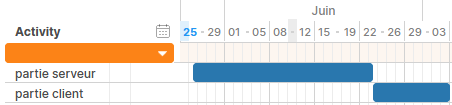
\includegraphics{img/gantt}
				\caption{Diagramme de Gantt du projet}
				\label{fig:gantt}
			\end{center}
		\end{figure}

	\section{Organisation}
		Les membres de l’équipe s’organiseront chaque jour sur les tâches faites et à faire via Discord. 

		Le projet étant découpé en beaucoup de fichiers, les membres du projet utiliseront une méthode de développement agile afin de développer chaque fonctionnalité indépendamment l’une de l’autre. Les membres de l’équipe ayant les mêmes compétences techniques, chacun pourra donc commencer le développement d’une nouvelle fonctionnalité lorsqu’il en aura terminé une. 

\chapter{Gestion des risques} 
	\bgroup
	\def\arraystretch{2}%  1 is the default, change whatever you need
	\begin{tabularx}{\textwidth}{|X|X|}
		\hline
		\LARGE Problème & \LARGE Solution \\
		\hline
		Perte de code via une mauvaise manipulation & 	Logiciel de versionning, copie locale chez chaque membre de l’équipe \\
		\hline
		Membre du groupe dans l’incapacité de travailler & Les membres de l’équipe possèdent les mêmes connaissances. Quelques fonctionnalités peuvent tout de même être abandonnées car l’avancement du projet en sera ralenti. \\
		\hline
		GitHub indisponible & Copie locale chez chaque membre de l’équipe \\
		\hline
		Discord indisponible & Autres moyens de communication : téléphone, mails \\
		\hline
	\end{tabularx}
	\egroup

\newpage
\phantomsection
\section*{Annexes}
\addcontentsline{toc}{chapter}{Annexes}

\begin{figure}[h]
	\begin{center}
		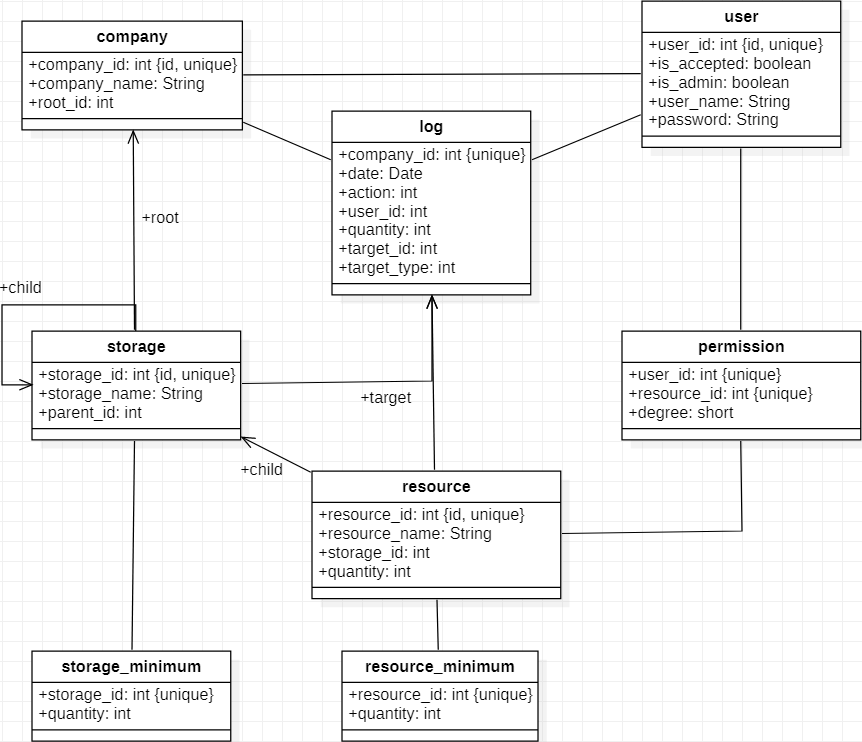
\includegraphics[scale=0.65]{img/UML}
		\caption{Diagramme UML de la base de données}
		\label{fig:UML}
	\end{center}
\end{figure}

%ends writting in the document
\end{document}